\chapter{Increased memory bandwidth}

Line $29$ of the function \texttt{MLDU\_Simple\_cell} is the obvious bottleneck of the implementation. This line gets called every iteration of the \texttt{for} loop and adds data to the matrix \texttt{A}. This addition of data requires many memory operations, which makes it slow. The performance of the main memory subsystem of a computer is comprised of two aspects, bandwidth and latency. Bandwidth is a measure of maximum throughput and latency is a measure of the access time.\\

\noindent This chapter tries to shed some light on which of the two main memory performance indicators is to blame for the poor performance of line $29$.

\section{GPU}

The GPU is interesting in this scenario because dedicated GPU's contains VRAM. Comparing VRAM to standard RAM, which makes up the main memory of a computer, reveals that VRAM has a much higher bandwidth than RAM. The downside is that VRAM has a somewhat higher latency than RAM.\\

\noindent Implementing the block MLDU algorithm on the GPU would make it possible to identify whether latency or bandwidth is to blame for the poor runtime of line $29$. A bandwidth bottleneck would result in a faster execution of line $29$ and a latency bottleneck would cause it to be slightly slower then on the CPU.

\section{MATLAB Sparse gpuArray limitations}

MATLAB facilitates GPGPU programming, but has limitations, especially when it comes to sparse matrices. The most notable limitations for the block MLDU algorithm are the inability to index in sparse gpuArrays and the fact that the "\textbackslash" operator is not feature complete.\\

\noindent These limitations make it very unappealing to write a "simple" MATLAB implementation of the block MLDU algorithm on the GPU. The overall performance will almost certainly be slower than the CPU implementation, because all the hacks required to get it functional will swamp any floating point performance benefits that the GPU has over the CPU.\\

\noindent Regardless, it will provide insight into the latency versus bandwidth question and as such is still valuable to this project.

\newpage

\subsection{The code}

\lstinputlisting{code/MLDU_Simple_GPU.m}

\subsection{Profiler results}

\noindent The profiler results below are generated by running:\\

\noindent \texttt{[ E ] = Test\_Function\_1( 40, @MLDU\_Simple\_GPU )}\\

\noindent The total runtime of this reduced size test was about $16$ seconds, which is way slower than the \texttt{MLDU\_Simple\_cell} implementation, which takes about $0.4$ seconds. The error of \texttt{MLDU\_Simple\_GPU} was again reasonable at $2.9072e-14$.

\begin{figure}[h!]
    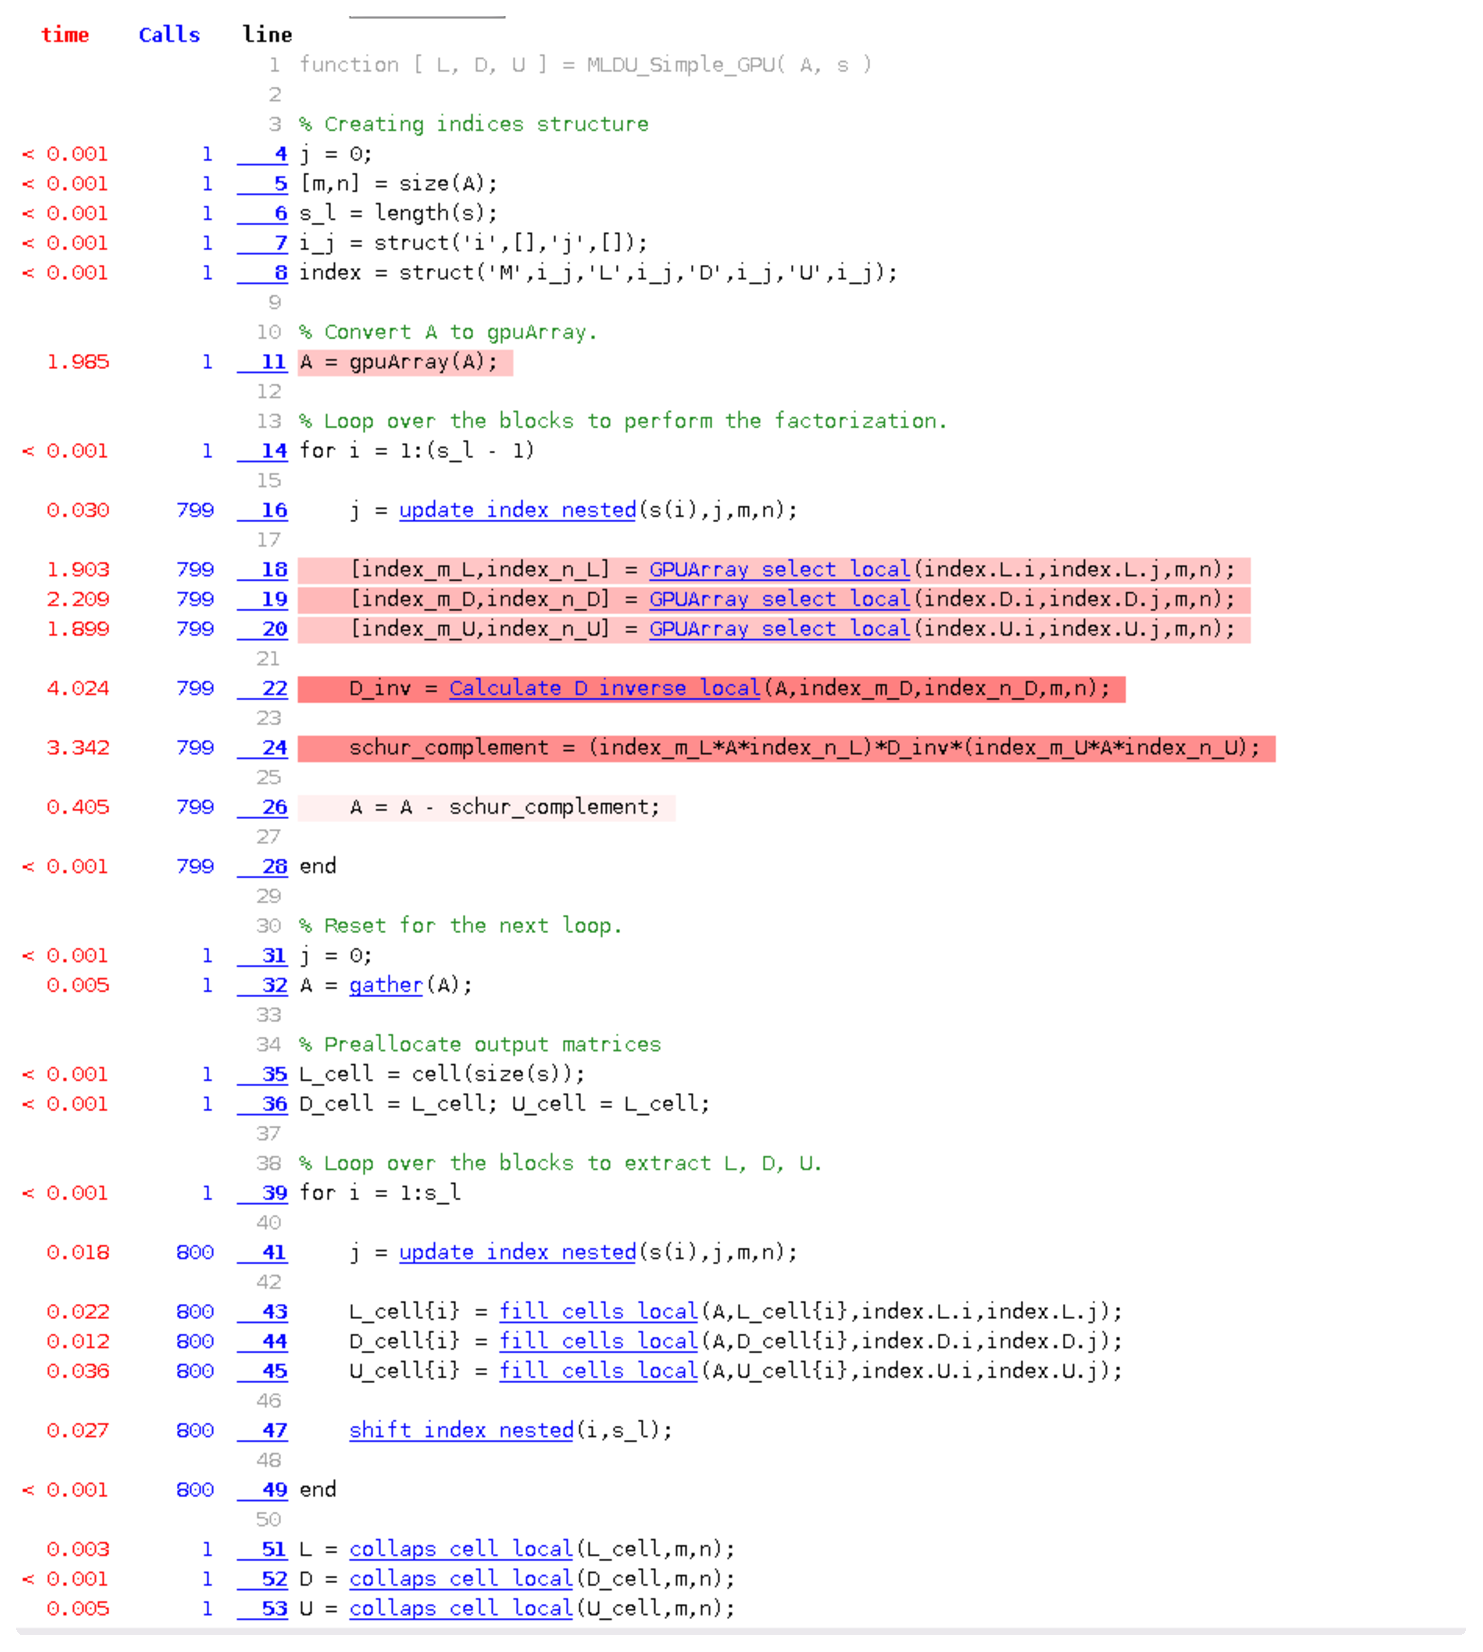
\includegraphics[width=\linewidth]{figures/Profile_MLDU_Simple_GPU_1.eps}
    \centering
\end{figure}

\newpage

\noindent The most interesting timing result for this discussion is that of line $26$ (above), which has a value of $0.405$. Line $29$ of \texttt{MLDU\_Simple\_cell} executes the same operation, but takes only $0.164$ seconds.\\

\noindent The profiler results of \texttt{[ E ] = Test\_Function\_1( 40, @MLDU\_Simple\_cell )} are provided below:

\begin{figure}[h!]
    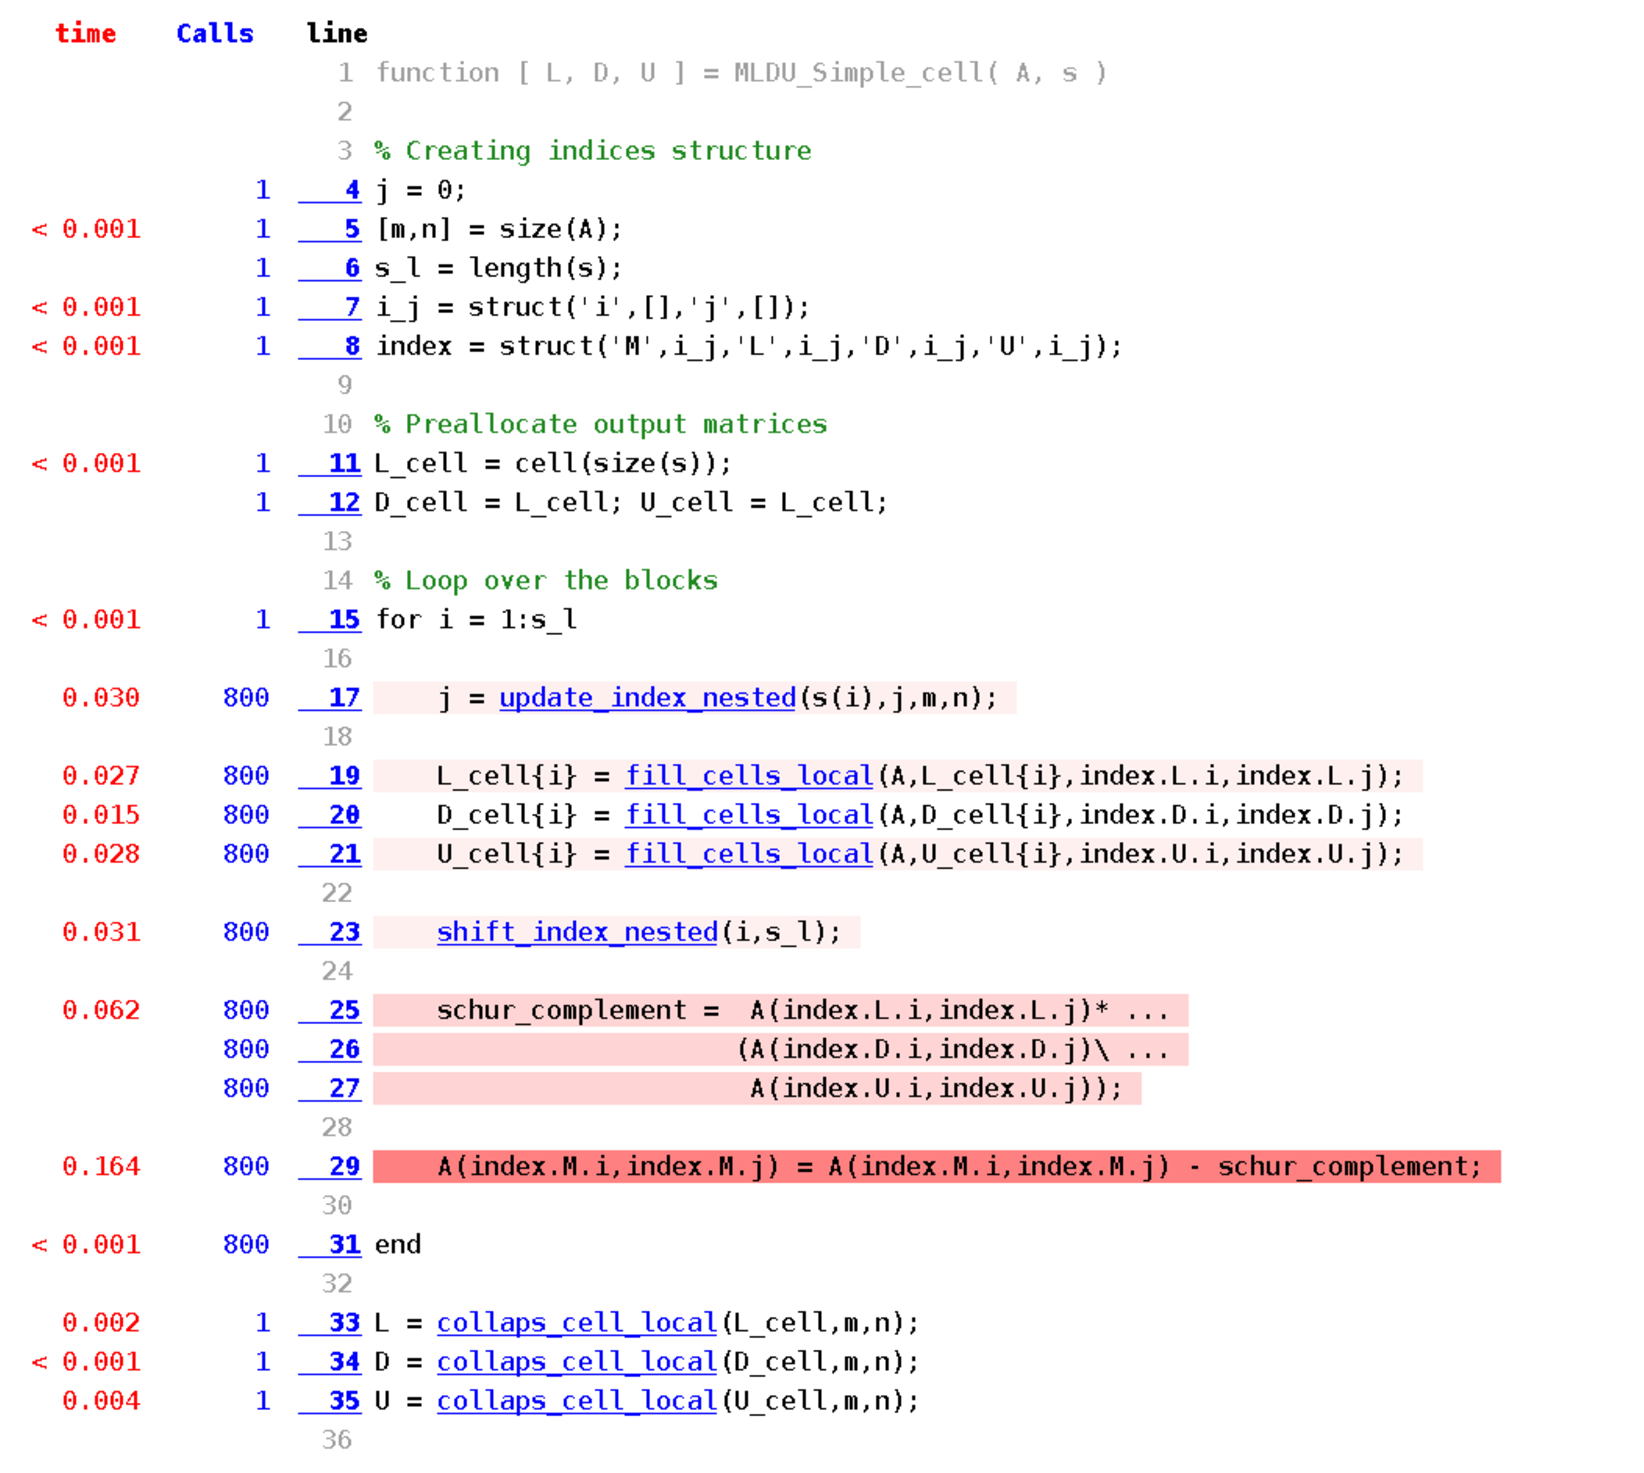
\includegraphics[width=\linewidth]{figures/Profile_MLDU_Simple_GPU_2.eps}
    \centering
\end{figure}

\noindent The clear result from \texttt{MLDU\_Simple\_GPU} is that it does not constitute an improvement. This may very well be down to the limiting aspects of MATLAB sparse gpuArrays, but further investigation would be required to know for certain. The second lesson from \texttt{MLDU\_Simple\_GPU} is that the operation at line $29$ or $26$ is latency bound.